\section{Phân chia chu kỳ hoạt động: phần điều khiển vs. phần truyền tải}

Như đã nói, mỗi slot $T$ được chia thành phần điều khiển ($\tau$) và phần truyền dữ liệu ($T-\tau$)
. Hình 2 minh họa chi tiết cấu trúc một slot với 4 giai đoạn: (a) Signaling – khởi tạo (Initialization), (b) Algorithmic (chạy thuật toán như CE, RA), (c) Signaling – thiết lập (Setup), và (d) Payload
\cite{ris_latency}
. Trong đó, ba giai đoạn đầu diễn ra trong khoảng thời gian điều khiển $\tau$, còn giai đoạn (d) chiếm phần còn lại $T-\tau$
. Công thức (13) biểu thị: $\tau = \tau_\text{ini} + \tau_\text{alg} + \tau_\text{setup}$, với $\tau_\text{ini}, \tau_\text{alg}, \tau_\text{setup}$ lần lượt là độ dài các pha Initialization, Algorithmic, Setup
.

\begin{figure}[H]
  \centering
  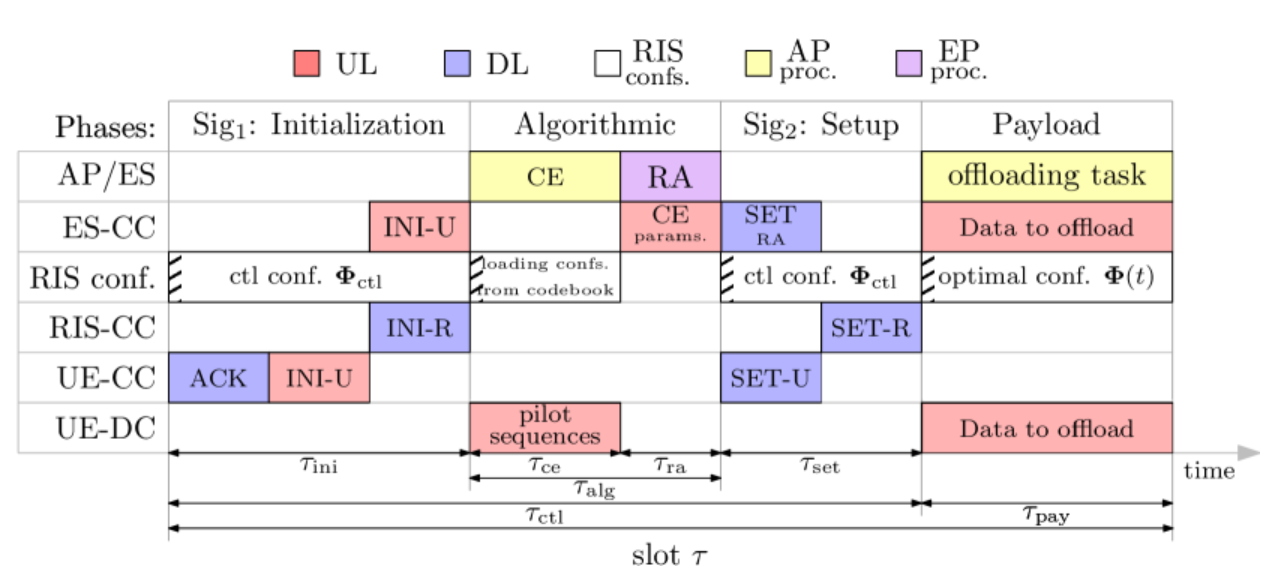
\includegraphics[width=1\textwidth]{images/f2.png}
  \caption{Sơ đồ thời gian một slot $t$. }
    \label{fig:my-image}
\end{figure}


Pha (a) Khởi tạo (Initialization): Mở đầu mỗi slot, AP và UE thực hiện thủ tục đồng bộ và chuẩn bị thông tin ban đầu. Cụ thể, AP gửi các bản tin ACK/NACK tới từng UE (thông báo UE biết dữ liệu gửi ở slot trước có nhận thành công không)
. Mỗi UE khi nhận NACK sẽ phải giữ lại dữ liệu chưa gửi thành công đó ở đầu hàng đợi để gửi lại, còn ACK thì có thể gỡ dữ liệu đã gửi ra khỏi hàng đợi
. Sau đó, mỗi UE gửi một gói điều khiển INI-U (Initialization-UE) lên AP thông qua kênh UE-CC UL, mang thông tin trạng thái hàng đợi của UE (ví dụ độ dài hàng đợi còn lại)
. AP thu thập các INI-U từ các UE và chuyển tiếp thông tin này tới ES qua kênh ES-CC
. Đồng thời, AP cũng gửi một gói INI-R (Initialization-RIS) tới RIS qua kênh RIS-CC để báo RIS chuẩn bị thực hiện ước lượng kênh
\cite{ris_latency}
. Cụ thể, lệnh INI-R yêu cầu RIS chuyển sang cấu hình điều khiển “ctl” – cấu hình pha đặc biệt có búp sóng rộng để phục vụ cho quá trình pilot (sẽ nói ở pha b)
. Trước khi RIS đổi sang cấu hình mới, cần một khoảng thời gian bảo vệ (guard period) do hạn chế phần cứng (ví dụ RIS cần vài micro-giây để thiết lập pha)
. Pha Initialization do đó bao gồm: thời gian phát các gói ACK (có thể đồng thời tới nhiều UE), thời gian UE gửi INI-U (có thể đồng thời nếu khác tần số do FDM), thời gian AP gửi INI-R (1 gói đơn), và thời gian guard chuyển cấu hình RIS. Công thức

\begin{equation}\label{eq:tau_ini}
\tau_{\mathrm{ini}} = \tau_{s} + 3T.
\end{equation}

mô tả tổng overhead thời gian cho pha Initialization $\tau_\text{ini}$, bao gồm các thành phần như trên
. Như vậy, $\tau_\text{ini}$ tỉ lệ với thời lượng gói điều khiển và thường khá nhỏ (vài TTI) nhưng không thể bỏ qua.


Pha (b) Thuật toán (Algorithmic): Đây là phần chính yếu của overhead, gồm hai quy trình: ước lượng kênh (CE) và tính toán phân bổ tài nguyên (RA).
\begin{itemize}
    \item Ước lượng kênh (CE): Nhằm biết được thông tin kênh CSI để tối ưu cấu hình, trong mỗi slot hệ thống phải dành thời gian cho UE gửi tín hiệu pilot. Với RIS, việc ước lượng phức tạp hơn do phải ước lượng cả kênh trực tiếp UE–AP lẫn kênh phản xạ qua RIS. Phương pháp phổ biến là sử dụng một bộ cấu hình RIS thử nghiệm (CE codebook) gồm $Q$ cấu hình khác nhau, lần lượt thiết lập RIS qua từng đợt pilot, để thu được $Q$ tín hiệu phản xạ, từ đó suy ra các thành phần kênh tương ứng
\cite{ris_latency}
. Cụ thể, trong bài báo, giả sử mỗi UE gửi một chuỗi pilot có độ dài $L$ TTI để ước lượng kênh trực tiếp (trong khi RIS tắt hoặc ở trạng thái mặc định), sau đó RIS lần lượt áp $Q$ cấu hình khác nhau và UE lặp lại chuỗi pilot $L$ TTI cho mỗi cấu hình. AP sẽ thu được $Q+1$ tín hiệu để tính ra kênh trực tiếp $h_{d}$ và $Q$ kết hợp $h_r$ tương ứng, từ đó suy luận kênh RIS–AP và UE–RIS riêng biệt
. Quá trình này diễn ra đồng thời cho tất cả UE (do FDM, mỗi UE ở băng riêng nên không nhiễu nhau)
. Giả sử $N$ phần tử RIS và kỹ thuật ước lượng cho phép nhóm các phần tử hoặc có độ suy giảm tự do, $Q$ có thể nhỏ hơn $N$ nhiều (các nghiên cứu CE cho RIS đề xuất $Q$ tỉ lệ $N$ hoặc $\log N$ tùy phương pháp
). Công thức cho thấy thời gian overhead CE là: $\tau_\text{CE} = L \cdot (1 + Q) + Q \cdot t_\text{switch}$
ar5iv.labs.arxiv.org
. Trong đó $t_\text{switch}$ là thời gian chuyển cấu hình RIS giữa các lần, nhân với $Q$ lần chuyển
. Rõ ràng, $\tau_\text{CE}$ tăng tỷ lệ với số cấu hình pilot $Q$. $Q$ càng lớn (kênh phức tạp, nhiều phần tử) thì overhead càng cao, bù lại CSI đầy đủ hơn. Nếu muốn giảm overhead, có thể giảm $Q$ nhưng khi đó thông tin kênh ít đi, có thể buộc hệ thống chấp nhận cấu hình RIS chưa tối ưu hoặc sử dụng thuật toán khác (như beam sweeping thay vì CE chính xác
).
    \item Tính toán phân bổ tài nguyên (RA): Sau khi có CSI (tạm coi đã có sau bước CE), máy chủ ES sẽ giải một bài toán tối ưu nhằm quyết định: cấu hình pha RIS tối ưu $\Phi^*(t)$ cho slot này, vector beamforming tại AP, phân bổ công suất cho mỗi UE, tần số CPU phục vụ mỗi UE, v.v., thỏa mãn các ràng buộc (như giới hạn năng lượng, đảm bảo trễ) và tối ưu hóa mục tiêu (như trễ trung bình nhỏ nhất hoặc năng lượng tiêu thụ tổng nhỏ nhất). Bài toán này thường phi tuyến và phức tạp, nhưng có thể giải bằng các thuật toán gần đúng (heuristic) hoặc tối ưu lồi hóa. Thuật toán được thực thi tại ES (hoặc AP) trong mỗi slot, do đó tiêu tốn thời gian tính toán – cũng chính là một phần overhead. Ký hiệu $\tau_\text{RA}$ là thời lượng ES/AP cần để hoàn tất thuật toán RA. Công thức (19) liên hệ $\tau_\text{RA} = \frac{C_\text{RA}}{f_\text{ES}}$ chẳng hạn, với $C_\text{RA}$ là số chu kỳ CPU cần để giải bài toán RA và $f_\text{ES}$ là xung nhịp CPU ES (chu kỳ/s) . Nếu ES dành một phần năng lực CPU cho RA song song với xử lý tác vụ thì có thể phức tạp; ở đây ta coi RA được ưu tiên làm trước rồi mới xử lý tác vụ. Từ giải thuật cụ thể, tác giả ước tính $C_\text{RA}$. Chẳng hạn, họ dùng thuật toán tham lam để tìm cấu hình RIS và beamforming AP tối ưu: cố định một vector beam tại AP, sau đó chọn dần cấu hình pha từng nhóm phần tử RIS sao cho cải thiện mục tiêu nhiều nhất . Số lựa chọn có thể duyệt cho một nhóm $g$ phần tử là $2 \times (2^b)^g$ (mỗi phần tử có 2 trạng thái: hoạt động hoặc tắt, và nếu hoạt động thì có $2^b$ mức pha lượng tử với $b$ bit phân giải) . Thuật toán lặp qua nhiều nhóm cho đến khi xét đủ $N$ phần tử hoặc đạt ngưỡng. Nếu chọn nhóm $g$ lớn (tức tối ưu theo cụm phần tử), độ phức tạp giảm nhưng hiệu quả giảm; nhóm $g=1$ (tối ưu từng phần tử) cho hiệu năng cao nhất nhưng phức tạp nhất . Cuối cùng, (20) đưa công thức tính số chu kỳ cần thiết $C_\text{RA}$ dựa trên số phép nhân phải thực hiện khi thử các khả năng . Kết luận: $\tau_\text{RA}$ càng lớn nếu bài toán phức tạp (nhiều biến như nhiều phần tử RIS) hoặc CPU chậm. Do đó, overhead điều khiển có thể giảm bằng cách giảm độ tối ưu (ví dụ nhóm nhiều phần tử RIS để giảm vòng lặp tính toán, chấp nhận cấu hình sub-optimal) .
\end{itemize}

Tổng thời gian pha Algorithmic là $\tau_\text{alg} = \tau_\text{CE} + \tau_\text{RA}$. Đây thường là phần chiếm nhiều nhất trong $\tau$.

Pha (c) Thiết lập (Setup): Sau khi ES tính toán xong các tham số tối ưu (công suất, tốc độ mã hóa, cấu hình RIS,...), AP sẽ gửi các thông tin thiết lập này trở lại UE và RIS để áp dụng trong phần truyền data của slot hiện tại  . Cụ thể, AP gửi gói SET-U cho từng UE chứa các tham số như: hệ số công suất $p_k(t)$ mà UE nên dùng, tốc độ dữ liệu (hoặc MCS – modulation and coding scheme) tối đa UE được phép truyền (dựa theo kênh ước lượng)  . Gói SET-U có thể gửi đồng loạt (broadcast hoặc multicast) nếu gọn, hoặc lần lượt nếu trễ cho phép. Đồng thời, AP gửi gói SET-R cho RIS chứa cấu hình pha tối ưu $\Phi^*(t)$ cần thiết lập  . Trước khi gửi SET-R, AP yêu cầu RIS chuyển sang chế độ nhận lệnh (thường RIS phải tạm thời về cấu hình “ctl” để dễ nhận tín hiệu điều khiển) – do đó cũng cần một khoảng guard ngắn để RIS chuyển trạng thái như ban đầu  . Tổng thời gian pha Setup $\tau_\text{setup}$ gồm thời gian phát các gói SET-U (có thể đồng thời trên nhiều tần số) + thời gian phát 1 gói SET-R + guard chuyển RIS về chế độ nhận lệnh. Công thức $\tau_\text{setup}$ gồm các thành phần đó.\cite{ris_latency}


Sau khi pha c) kết thúc, RIS có cấu hình mới $\Phi^*(t)$, các UE biết mình sẽ truyền bao nhiêu với công suất bao nhiêu, AP/ES sẵn sàng thu và xử lý – hệ thống chuyển sang pha (d) truyền dữ liệu (Payload) trong thời gian $T-\tau$. Tại đây, mỗi UE gửi một phần dữ liệu (có thể là toàn bộ hàng đợi nếu đủ thời gian) qua kênh UL. Nhờ có RIS điều chỉnh tối ưu và AP biết trước công suất truyền, việc tiếp nhận sẽ hiệu quả. AP thu tín hiệu, gỡ lỗi; cuối slot AP chuyển dữ liệu thu được sang ES xử lý (có thể xử lý song song để giảm độ trễ). Vòng lặp tiếp tục cho slot tiếp theo.


Tóm lại, overhead $\tau$ mỗi slot gồm 3 pha: Khởi tạo, Thuật toán, Thiết lập. Overhead này không cố định mà phụ thuộc vào tham số hệ thống và thiết kế giao thức: số UE, độ dài gói điều khiển, số cấu hình pilot $Q$, độ phức tạp thuật toán RA, tốc độ phần cứng (RIS switching, CPU), v.v. Bảng 1 (giả định) tóm tắt đóng góp của từng yếu tố vào $\tau$. Chẳng hạn, nếu muốn giảm độ trễ, ta có thể giảm $Q$ (nhưng đánh đổi độ chính xác CSI), hoặc dùng thuật toán RA đơn giản hơn (đánh đổi hiệu năng). Phần sau chúng tôi sẽ phân tích kỹ sự đánh đổi này.
